\section{方法} 
\label{sec:proposed}

这一章节将对基于阈值的图像分割方法和本文所进行实验的基于直方图的自适应阈值分割进行介绍。

\subsection{基于阈值的图像分割方法}

图像分割旨在根据一定的准则将图像 $I$ 划分为不同区域的集合 $S$,集合 $S$ 满足下列条件:

\begin{enumerate}
	\item $\cup S_i = S$  
	\item $S_i \cap S_j=\emptyset,\;i \neq j$
	\item $\forall S_i,\; P(S_i)=true$
	\item $P(S_i\cup S_j)=false,\; i\neq j,\; S_i \; adjacent \; S_j$
\end{enumerate}
 
对于灰度图像而言,可以将其看作由目标(前景)和背景所构成,基于阈值的分割方法就是通过一个固定阈值将图像中的目标像素与背景像素进行分割,从而实现从图像中提取目标的目的。上述过程可以用下面的公式进行描述:

\begin{equation}
I'(x, y)=\left\{\begin{array}{l}
255, \;I(x, y)>\text{thresholding} \\[2em]
0, \;\quad I(x, y) \leq \text{thresholding}
\end{array}\right.
\vspace{0.5cm}
\end{equation}

其中,$\text{thresholding}$ 是设定的阈值,$x$ 与 $y$ 表示像素在图像中的坐标,$I(x, y)$ 为像素 $(x,y)$ 在原始图像中的灰度值,$I'(x, y)$ 为像素 $(x,y)$ 根据阈值分割后的二值图像对应的像素值。代码实现如下:
\vspace{0.3cm}
\lstinputlisting[language=Python,firstline=51,lastline=56]{main.py}

阈值的选择对于基于阈值的分割方法而言至关重要。在理想条件下,目标和背景的灰度值具有明显的划分,可以将直方图的峰值之间的数值设置为阈值。但在实际应用中,由于各种环境因素的影响,目标和背景的灰度值界限并不易于区分,如图 \ref{fig:random_thresholding} 所示,阈值设置过低时,背景中的噪声也会被划分到目标类别中,而当阈值设置过高时,目标中灰度值较低的部分被划入了背景部分。此外,对于不同的图像而言,相同的阈值也会取得不同的分割效果。因此,阈值的设置是基于阈值的分割方法的一大难题。图像分割阈值的设置常用方法包括:

\begin{itemize}
	\item 基于直方图形状:对去噪后的直方图的峰值、谷值和曲率等进行分析从而确定阈值
	\item 基于聚类:迭代找到阈值,并基于该阈值进行聚类
	\item 基于熵:选择一个使直方图信息量最大化的阈值
	\item 空间阈值(高阶统计):阈值的选择是基于空间邻域的高阶统计量
	\item 局部阈值:在每个邻域内利用局部统计信息寻找阈值
\end{itemize}

本文实验的方法是基于直方图的自适应阈值分割,即将图像的灰度直方图中的目标分量和背景分量分别参数化为模型(如高斯分布),然后在图像的灰度范围内迭代地设置不同的阈值,在当前阈值下,可以利用直方图的信息对模型中的未知参数进行估计(如高斯分布的均值、方差等),进而利用估计的参数对图像的整体灰度直方图进行“预测”。在同时具有“预测”分布和真实分布的情况下,就可以对不同阈值下“预测”的模型或分布进行评价,从而获得使拟合效果最好的阈值。

\subsection{基于直方图的自适应阈值分割}

图像的灰度直方图可以反映一幅图像中的灰度分布信息,能够为阈值的选取提供重要参考依据。基于直方图的自适应阈值分割方法,首先利用灰度直方图对图像的灰度分布进行统计,其实现利用了 matplotlib 包中的 pyplot.hist 接口。如图 \ref{fig:gray_level_histogram} 所示:

\begin{figure}[!ht]
\vspace{-0.9cm}
  \centering
  \begin{minipage}[b]{\linewidth} 
  \subfloat[]{
    \begin{minipage}[b]{0.36\linewidth} 
      \centering
      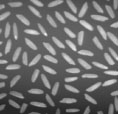
\includegraphics[width=\linewidth]{fig2_a}
     \end{minipage}
  }
  \hfill
    \subfloat[]{
    \begin{minipage}[b]{0.58\linewidth}
      \centering
      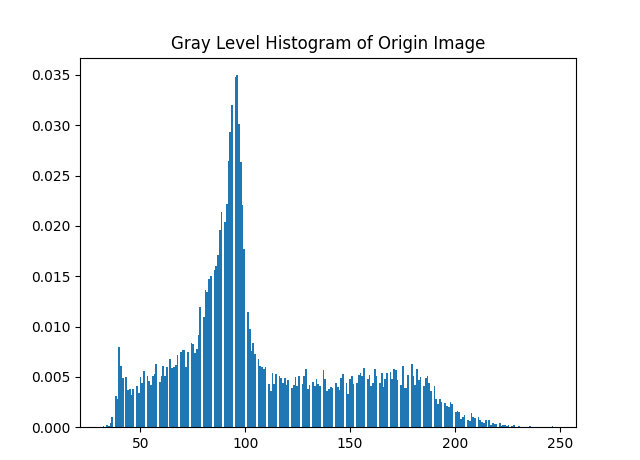
\includegraphics[width=\linewidth]{fig2_b}
       \end{minipage}
  }
  \end{minipage}
  \vfill
  \caption{Test\_Img\_1 及其灰度直方图:(a) 原始图像, (b) 灰度直方图.}
  \label{fig:gray_level_histogram}
\end{figure}

为了去除噪声的影响以及便于后续分布的拟合,要对直方图进行预处理,可以采用均值滤波或一维高斯滤波。本文采用了一维高斯滤波,结果如图 \ref{fig:smoothed_hist} 所示:

\begin{figure}[!ht]
%\vspace{-0.3cm}
	\centering
	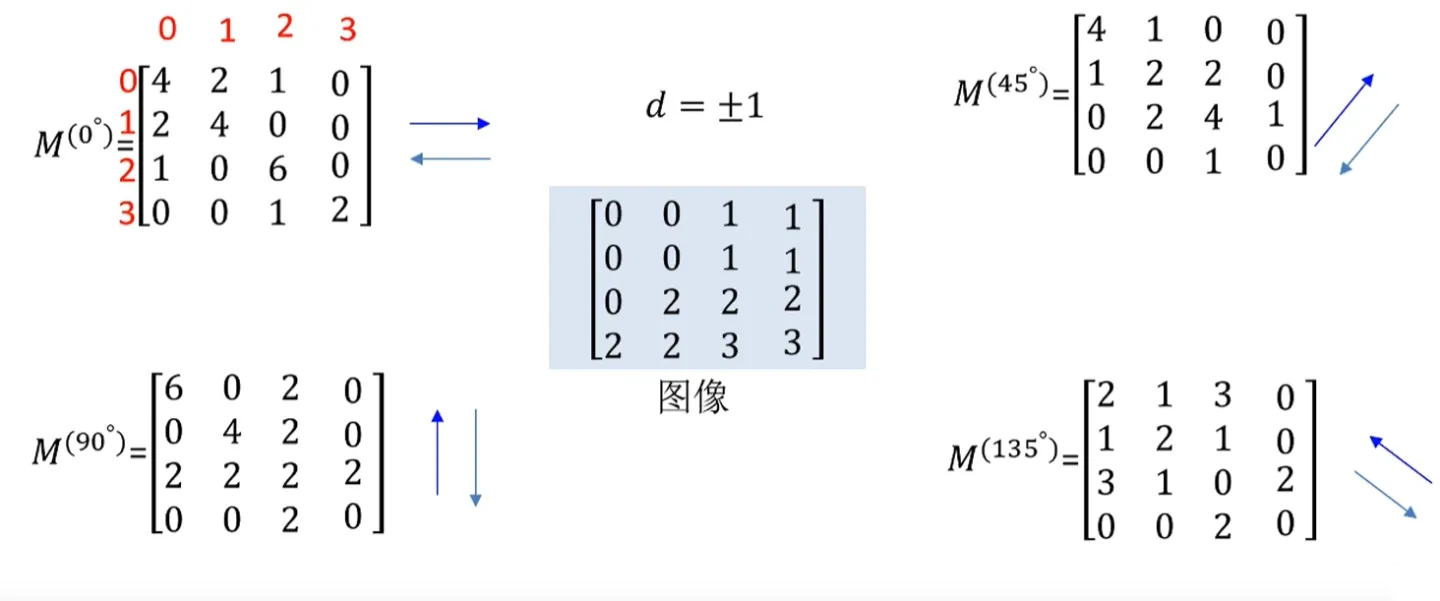
\includegraphics[width=\columnwidth]{fig3}
	\caption{Test\_Img\_1 经过一维高斯滤波后的灰度直方图曲线}
	\label{fig:smoothed_hist}
\end{figure}

一维高斯滤波的实现是通过生成一个滑动窗口大小的离散序列,该序列服从 0 均值,指定方差的高斯分布(不同的方差滤波的结果不同,方差越大,滤波的结果也越平滑)。然后利用该序列对原始灰度曲线做卷积,其代码实现如下:
\vspace{0.3cm}
\lstinputlisting[language=Python,firstline=43,lastline=48]{main.py}

为了对滤波处理后的灰度分布曲线进行拟合,同时将图像中的目标灰度值与背景灰度值进行区分,就需要分别建立符合目标和背景分量的直方图形状的参数模型,从图 \ref{fig:smoothed_hist} 可以看出,目标分量和背景分量的直方图形状近似于高斯分布,而图像整体的灰度直方图形状即为由两个高斯分布组成的混合高斯分布。因此,在基于直方图的自适应阈值分割方法中,用下面两个高斯分布来分别代表目标和背景的分布:

\begin{equation}
f_o(g)=\frac{1}{\sqrt{2 \pi} \sigma_o} e^{-1 / 2\left(\frac{g-\mu_o}{\sigma_o}\right)^2}
\end{equation}

\begin{equation}
f_b(g)=\frac{1}{\sqrt{2 \pi} \sigma_b} e^{-1 / 2\left(\frac{g-\mu_b}{\sigma_b}\right)^2}
\vspace{0.5cm}
\end{equation}

其中,$f_o(g)$ 和 $f_b(g)$ 分别为目标和背景的分布函数,同时也表示灰度值为 $g$ 的像素占图像总体像素的百分比,$\mu_o$ 和 $\mu_b$ 分别为目标和背景的灰度均值,$sigma_o$ 和 $sigma_b$ 分别为目标和背景的标准差。

高斯分布用 Python 实现的代码如下:
\vspace{0.3cm}
\lstinputlisting[language=Python,firstline=59,lastline=62]{main.py}

我们希望阈值可以将目标和背景的灰度分布进行分割,换句话来说,就是目标和背景的灰度可以分别分布在阈值的左右两侧。因此,我们可以假定一个阈值 $t$,然后对灰度图像直方图中阈值 $t$ 左右两侧的灰度信息进行统计计算,从而可以利用统计数据对 $f_o(g)$ 和 $f_b(g)$ 的均值及标准差进行估计,其估计方法如下所示:

\begin{equation}
\mu_o(t)=\sum_{g=0}^t f(g) g \quad \mu_b(t)=\sum_{g=t+1}^{\text {max }} f(g) g
\end{equation}

\begin{equation}
\sigma_o=\sum_{g=0}^t f(g) \left(g-\mu_o\right)  \quad \sigma_b=\sum_{g=t+1}^{\text {max }} f(g) \left(g-\mu_b\right)
\end{equation}

根据先验,我们可以得到一个像素落在目标或落在背景的概率分别为:

\begin{equation}
p_o(t)=\sum_t^{g=0} f(g)
\end{equation}

\begin{equation}
p_b(t)=1-p_o(t)
\vspace{0.5cm}
\end{equation}

对于假定的阈值 $t$,可以通过下面的公式对图像整体的灰度分布进行“预测”,并同样利用一维高斯滤波对估计的分布进行滤波处理:

\begin{equation}
P_t(g)=p_o f_0(g)+p_b f_b(g)
\vspace{0.5cm}
\end{equation}

上述过程的代码实现如下:
\vspace{0.3cm}
\lstinputlisting[language=Python,firstline=65,lastline=87]{main.py}

最后,只需要在图像的灰度值变化范围内对潜在的阈值进行迭代,并通过计算 KL 散度来度量“预测”分布与真实分布之间的相似性,从而搜索到使得二者最相似的阈值即可,KL 散度的计算公式为:

\begin{equation}
K(t)=\sum_{g=0}^{\max } f(g) \log \left[\frac{f(g)}{P_t(g)}\right]
\vspace{0.5cm}
\end{equation}

其 Python 代码为:
\vspace{0.3cm}
\lstinputlisting[language=Python,firstline=90,lastline=94]{main.py}

